%!TEX root = ../report.tex

\begin{document}
    \chapter{Results and Evaluation}

    In this chapter, the results of the registration of the available data using the solution presented in \autoref{chap:Solution} will be presented and discussed.
    The data was visualized and evaluated with the use of the 3D visualization provided by Open3D.

    The running times presented in \autoref{table:running_time} were taken on an Intel Core i7-1065G7 3.9GHz with 16 GB RAM.
    The most time-consuming task with the CityGML model is the detection of line segments.
    In comparison, the most time-consuming task with the PLY model is the alignment of both projections onto the xy-plane (the Mixed Integer Linear Program).

    These running times are obtained with the assumption that the position of the point cloud is not far away from the position of the 3D model, 
    as described in \autoref{sub:Identification of possible correspondences between angles detected}. 
    If this assumption is not considered, then the Mixed Integer Linear Program’s running time 
    is increased to 6.682 seconds for the CityGML model and 32.906 seconds for the PLY model.

    \begin{table}[h!]
        \centering
        \begin{tabular}{ |b{22em}|b{7em}|b{7em}| } 
            \hline
            \diagbox[width=23.2em]{Task}{Data} & CityGML model & PLY model \\ 
            %\diaghead{\theadfont Diag ColumnmnHead II}{Task}{Data}& CityGML model & PLY model \\ 
            \hline
            Projection onto the xy-plane & 0.607 s & 1.33 s \\ 
            \hline
            Detection of line segments & 3.198 s & 3.662 s \\ 
            \hline
            Detection of line intersections and their angles & 0.226 s & 0.229 s \\
            \hline
            Identification of possible correspondences & 0.005 s & 0.017 s\\
            \hline
            Alignment of both projections onto the xy-plane & 2.904 s & 14.359 s\\
            \hline
            Alignment on the z-axis & 0.421 s & 1.859 s\\
            \hline
        \end{tabular}
        \caption{Running time of the registration.}
        \label{table:running_time}
    \end{table}

%-------------------------------------------------------------------------------
%	Registration of a CityGML model with a point cloud
%-------------------------------------------------------------------------------
    \section{Registration of a CityGML model with a point cloud}
        The initial pose of the CityGML model and the point cloud can be found in \autoref{fig:initial_CityGML}.
        \autoref{fig:initial_front_model} shows a front view of the fire exercise building in Dortmund, while \autoref{fig:initial_back_model} shows a back view.
        The point cloud is just rotated around the z-axis and translated across the x- and y-axis.
        It is also slightly translated across the z-axis, but this is not easy to visualize.

        After the registration process, the resulting transformation is

        \begin{equation*}
            T_1 = 
            \begin{bmatrix}0.987 & -0.197 & 0.0 & -4.994 \\ 
                0.197 & 0.987 & 0.0 & -2.636 \\
                0.0 & 0.0 & 1.0 & -0.207 \\
                0.0 & 0.0 & 0.0 & 1.0
            \end{bmatrix}
        \end{equation*}

        and the results after applying this transformation to the point cloud are shown in \autoref{fig:final_CityGML}.
        In the transformation, one can observe a rotation around the z-axis and a translation across the x-, y-, and z-axis.

        \begin{figure}[htp]
            \centering
            \begin{subfigure}{1\textwidth}
                \centering
                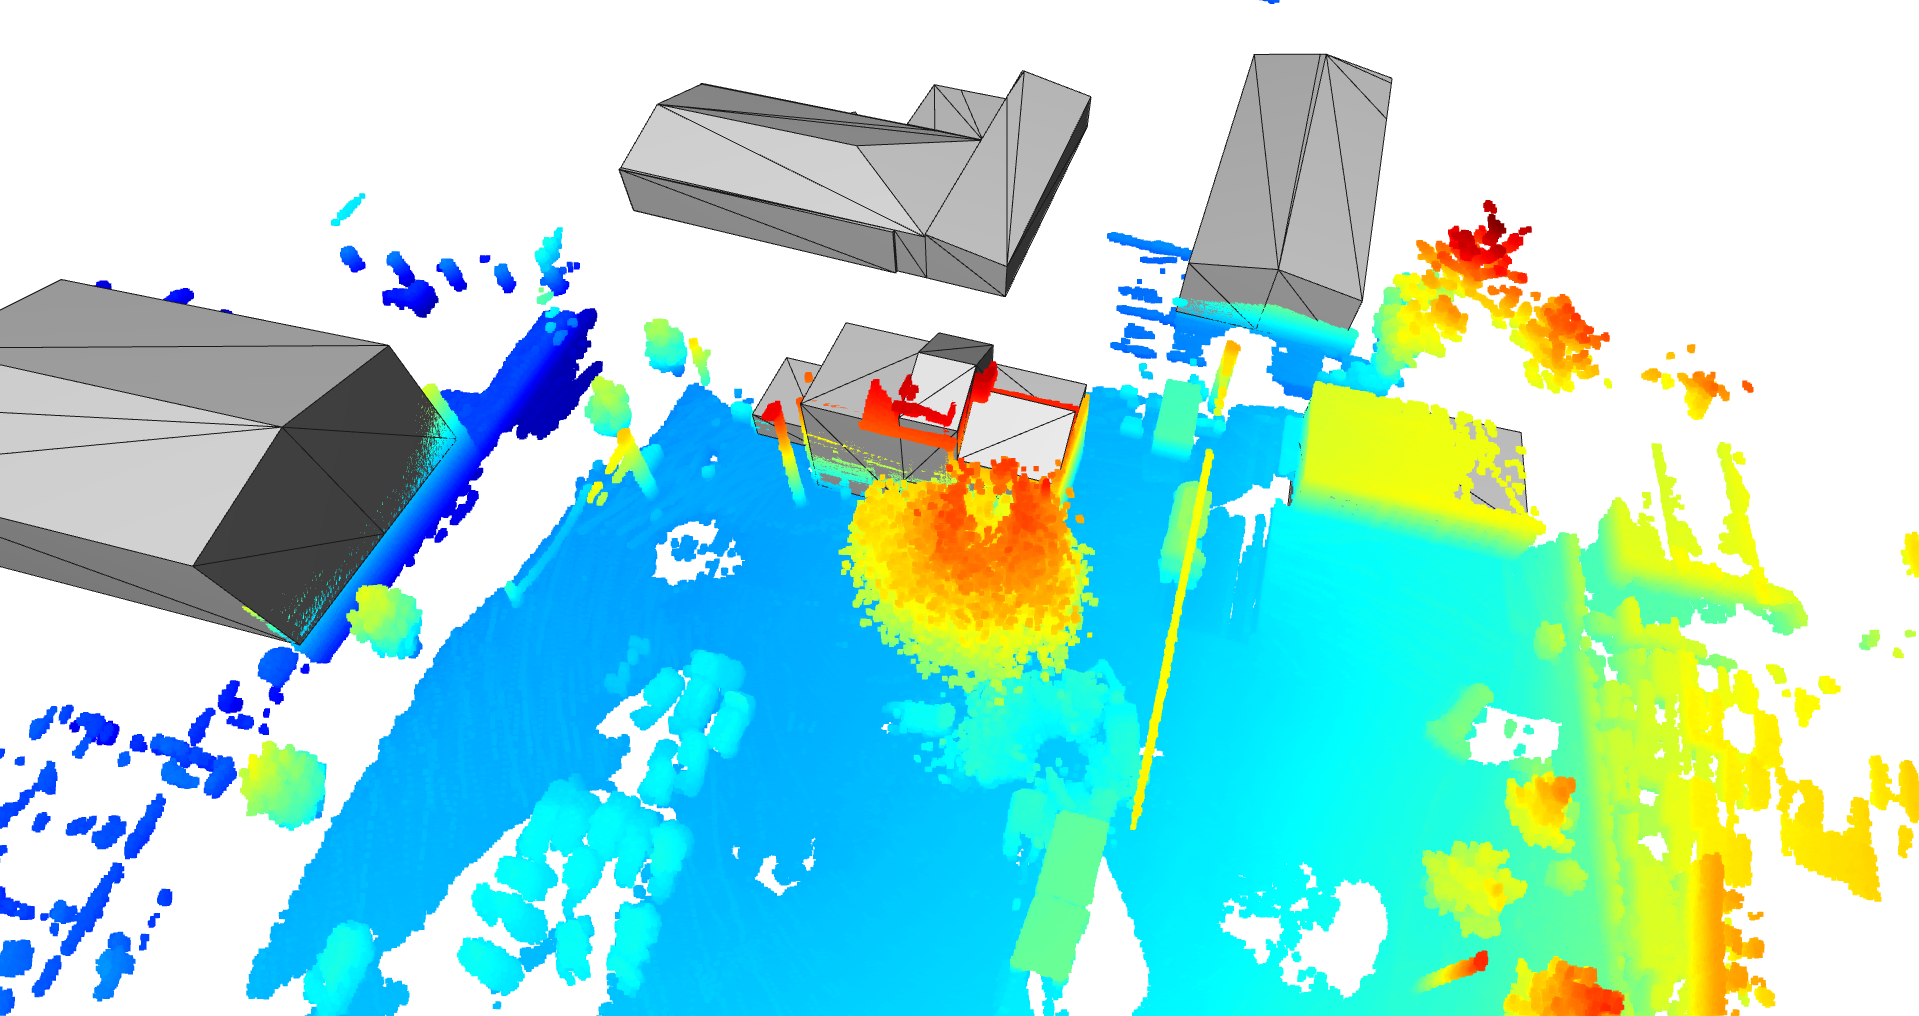
\includegraphics[scale=0.15]{images/solution_images/final_front.png}
                \caption{Front view.}
                \label{fig:final_front_model}
            \end{subfigure}
            \hfill
            \begin{subfigure}{1\textwidth}
                \centering
                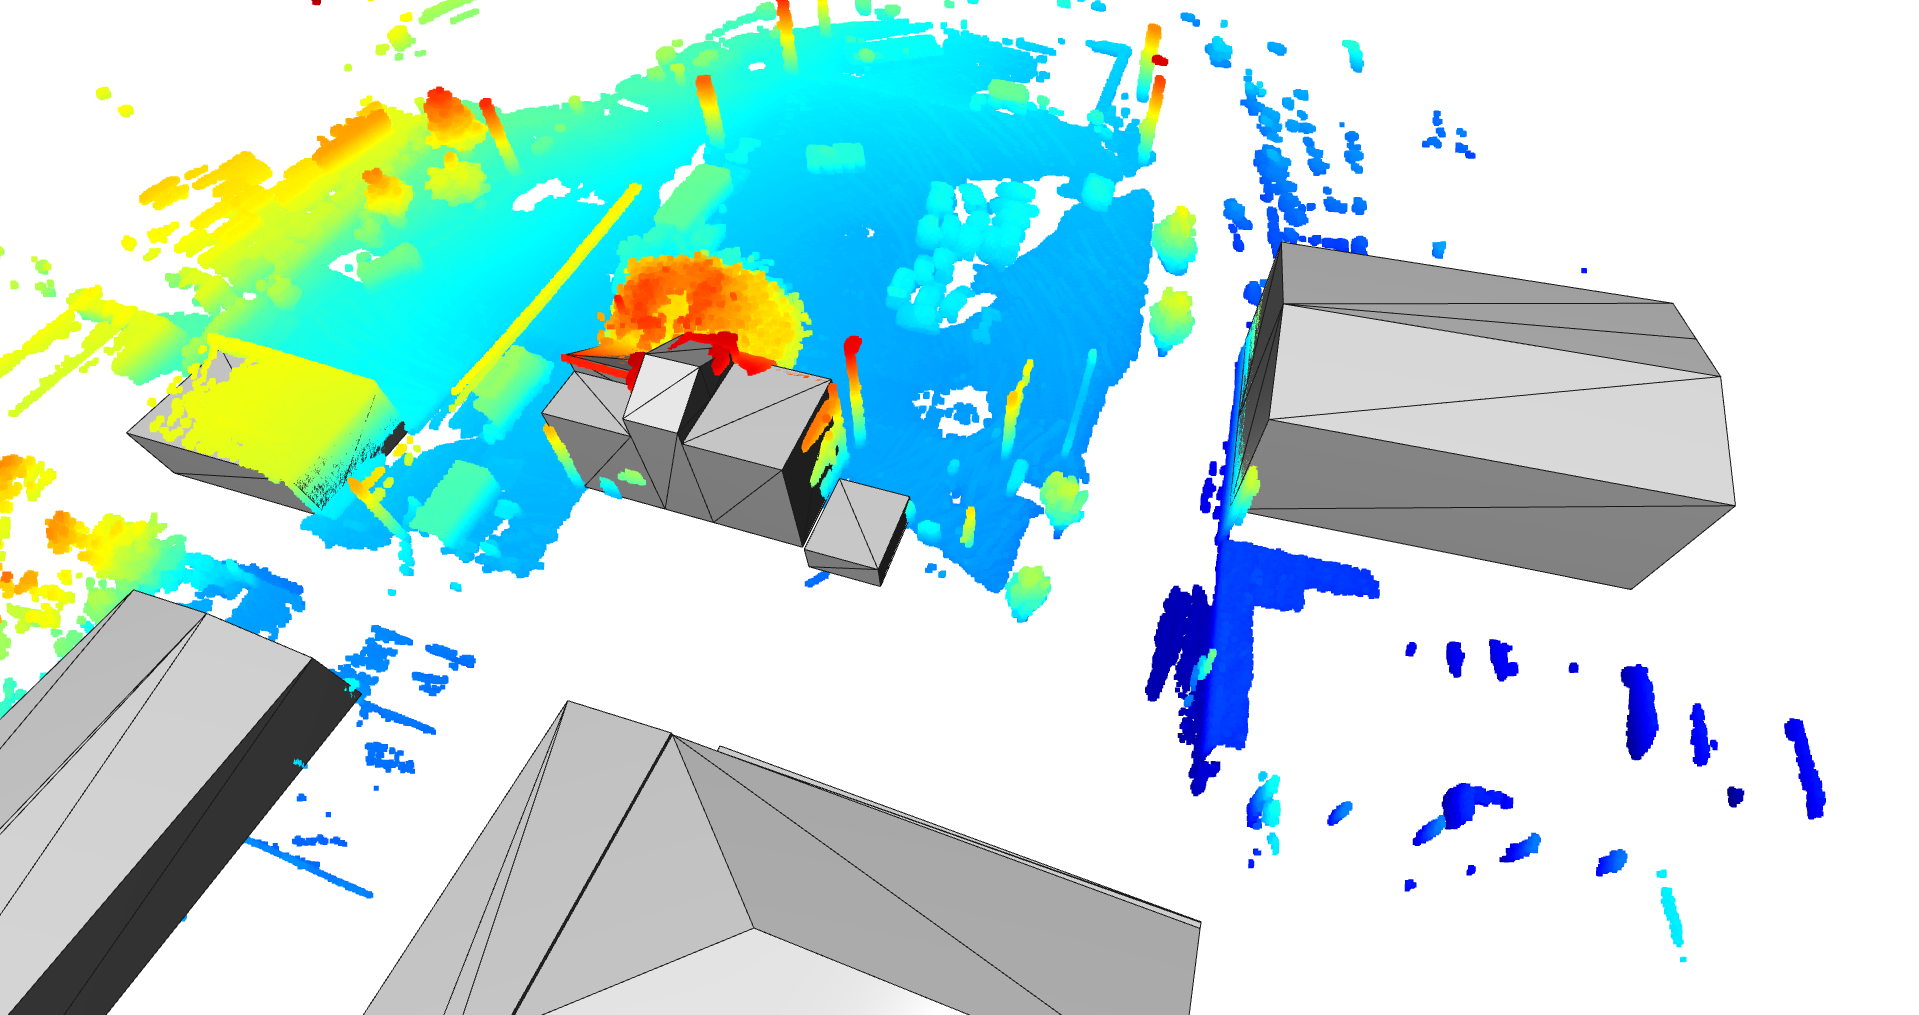
\includegraphics[scale=0.15]{images/solution_images/final_back.png}
                \caption{Back view.}
                \label{fig:final_back_model}
            \end{subfigure}
            \caption{CityGML model and its corresponding point cloud after registration.}
            \label{fig:final_CityGML}
        \end{figure}
        
        The alignment of the CityGML model with the point cloud can be seen in the fire exercise building (the one in the center of the image)
        and the right building in \autoref{fig:final_front_model}. The walls and the ceilings are correctly overlapped in both buildings.
        There is only a slight misalignment in the center part of the fire exercise building’s ceil because the CityGML model is outdated.

%-------------------------------------------------------------------------------
%	Registration of a PLY model with a point cloud
%-------------------------------------------------------------------------------
    \section{Registration of a PLY model with a point cloud}

        The second available data represents a part of the Technical University of Darmstadt.
        The 3D model is given in ply format, but this does not make any difference in the visualization.
        \autoref{fig:initial_ply} shows two different views of the initial pose of the 3D model and its corresponding point cloud.
        This time, the point cloud is translated across the x-, y-, and z-axis and rotated around the z-axis. 
        
        \begin{figure}[htp]
            \centering
            \begin{subfigure}{1\textwidth}
                \centering
                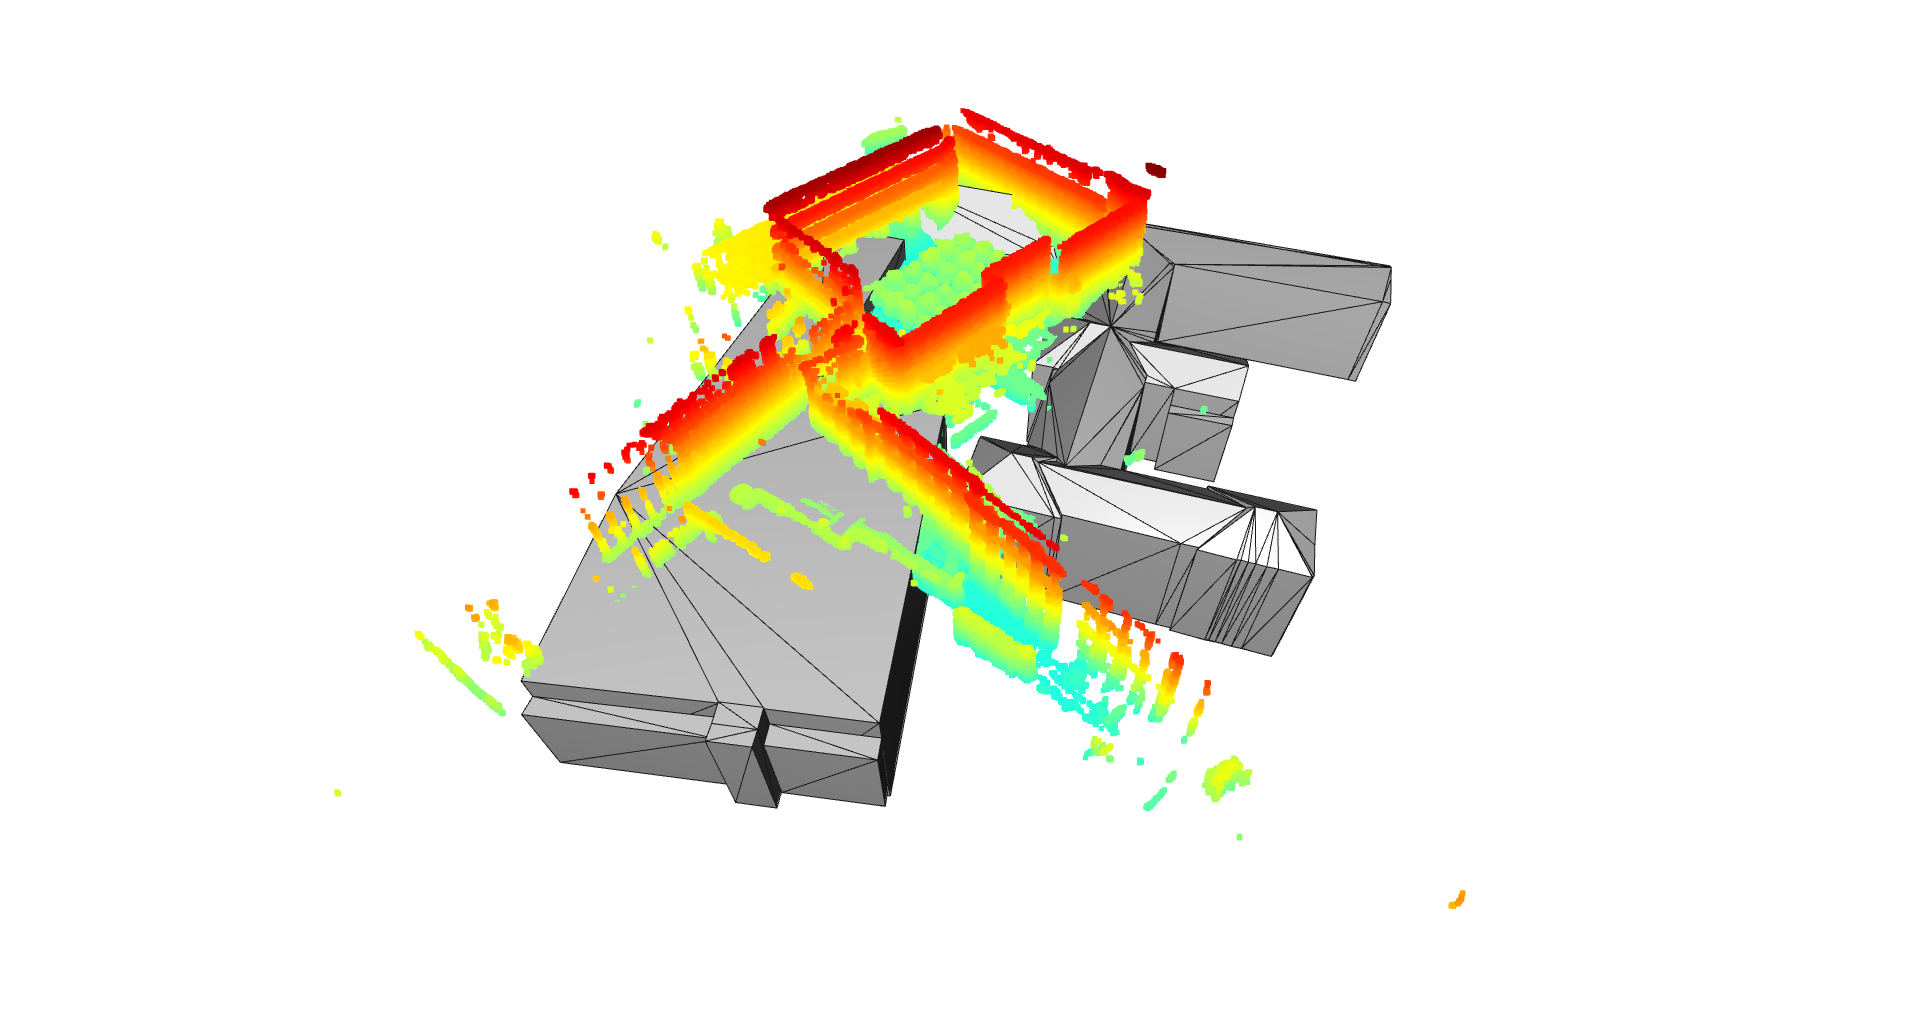
\includegraphics[scale=0.15]{images/solution_images/initial_ply_a.png}
                \caption{Frist view.}
                \label{fig:intial_ply_a}
            \end{subfigure}
            \hfill
            \begin{subfigure}{1\textwidth}
                \centering
                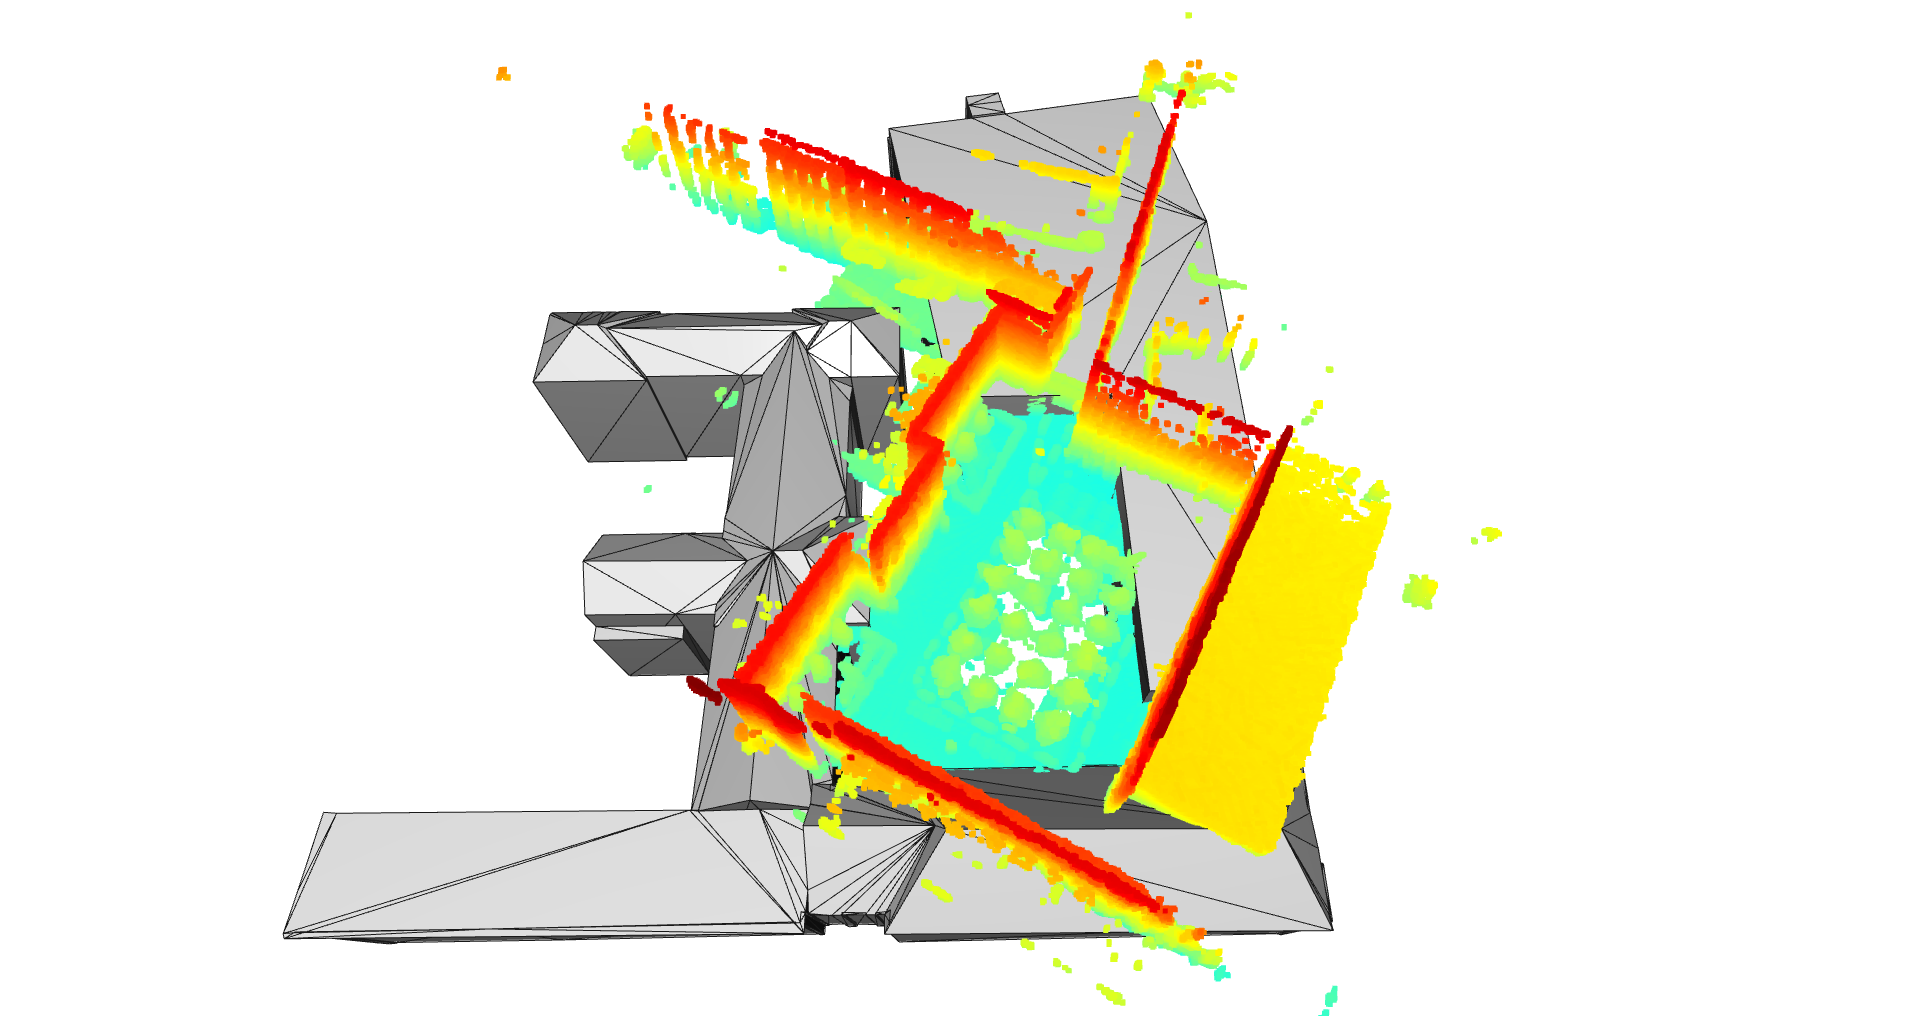
\includegraphics[scale=0.15]{images/solution_images/initial_ply_b.png}
                \caption{Second view.}
                \label{fig:intial_ply_b}
            \end{subfigure}
            \caption{PLY model and its corresponding point cloud before registration.}
            \label{fig:initial_ply}
        \end{figure}

        After the registration process, the resulting transformation is

        \begin{equation*}
            T_2 = 
            \begin{bmatrix}
                0.882 & -0.455 & 0.0 & 20.504 \\ 
                0.455 & 0.882 & 0.0 & -21.645 \\
                0.0 & 0.0 & 1.0 & -19.254 \\
                0.0 & 0.0 & 0.0 & 1.0
            \end{bmatrix}    
        \end{equation*}
        
        and the results after applying this transformation to the point cloud are shown in \autoref{fig:final_ply}.        

        In the transformation, one can observe a rotation around the z-axis and a translation across the x-, y-, and z-axis.
        This time, the translation across the z-axis is considerably larger than the one in $T_1$.

        In \autoref{fig:final_ply}, one can see that the walls are correctly aligned.
        Unfortunately, the point cloud does not contain any scans of the ceilings, and it is not clear whether the alignment in the z-axis is correct or not. 
        However, the point cloud contains the ground information of the center area between the buildings, 
        and one can see that it is aligned with the floor of the buildings.
        
        \begin{figure}[htp]
            \centering
            \begin{subfigure}{1\textwidth}
                \centering
                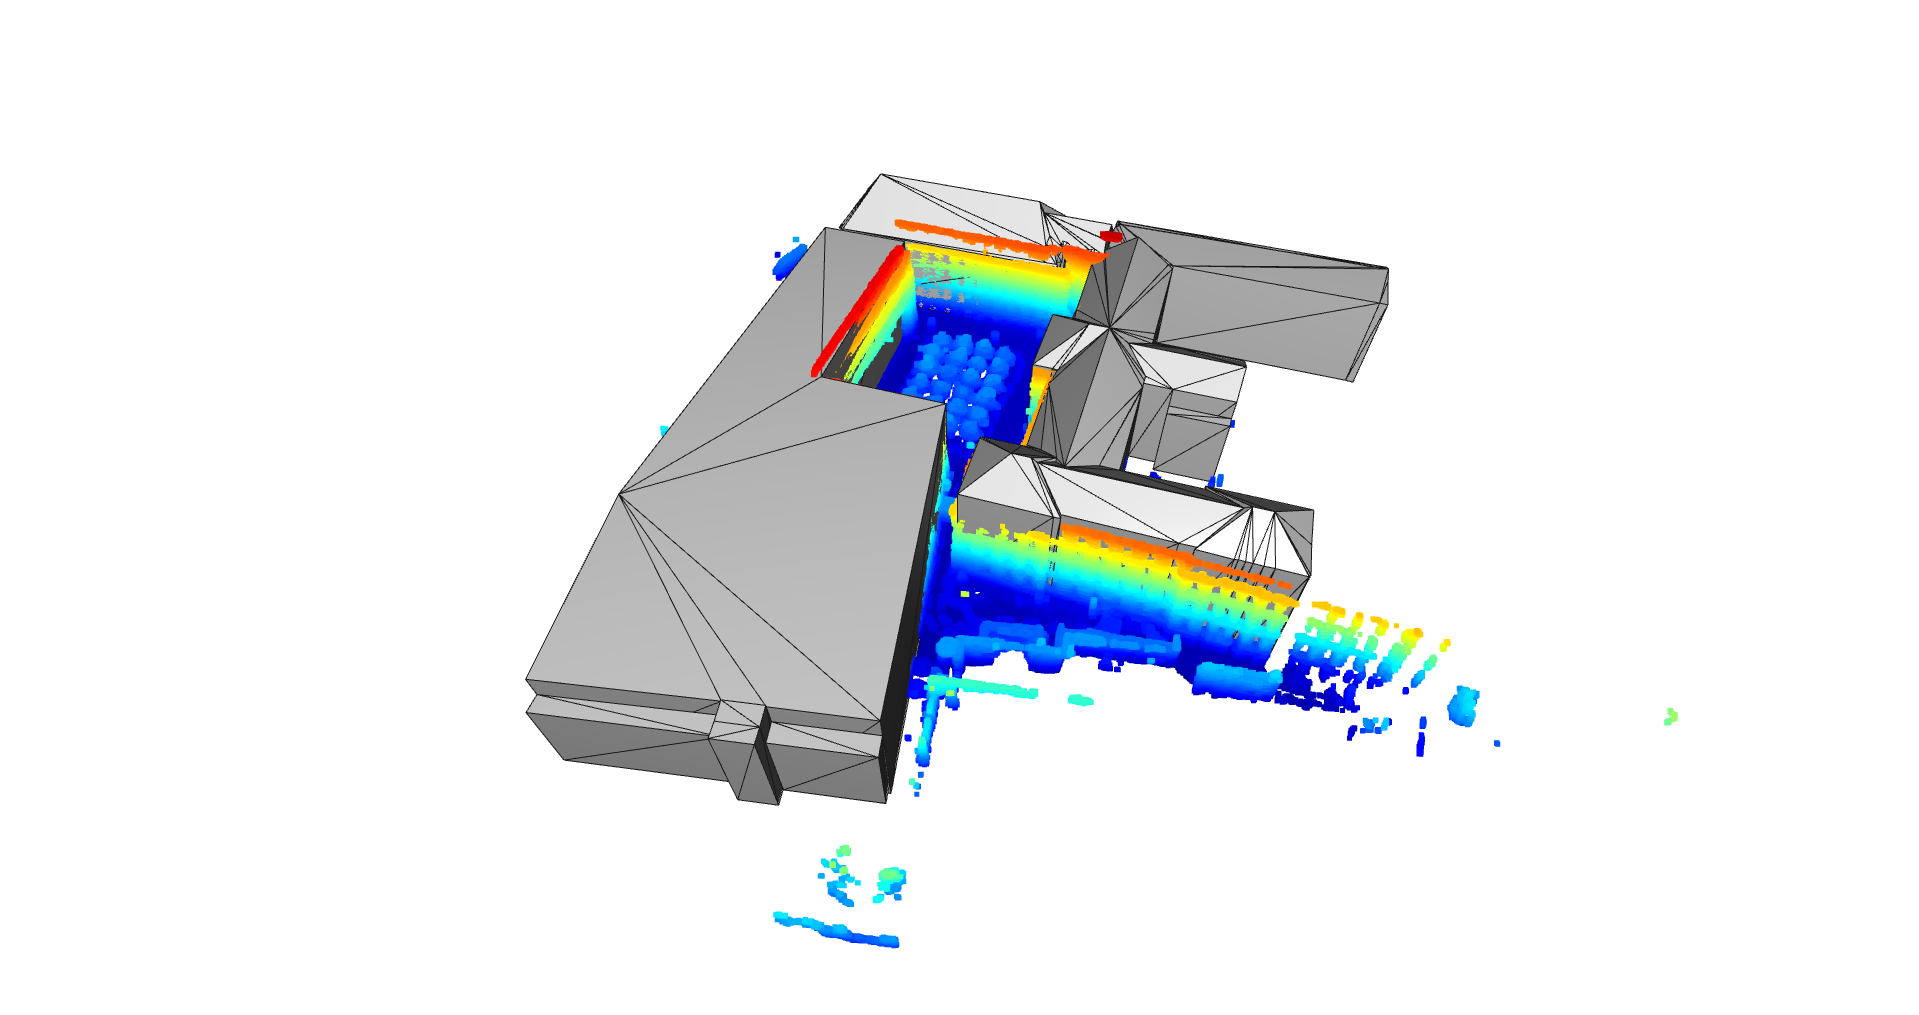
\includegraphics[scale=0.15]{images/solution_images/final_ply_a.png}
                \caption{First view.}
                \label{fig:final_ply_a}
            \end{subfigure}
            \hfill
            \begin{subfigure}{1\textwidth}
                \centering
                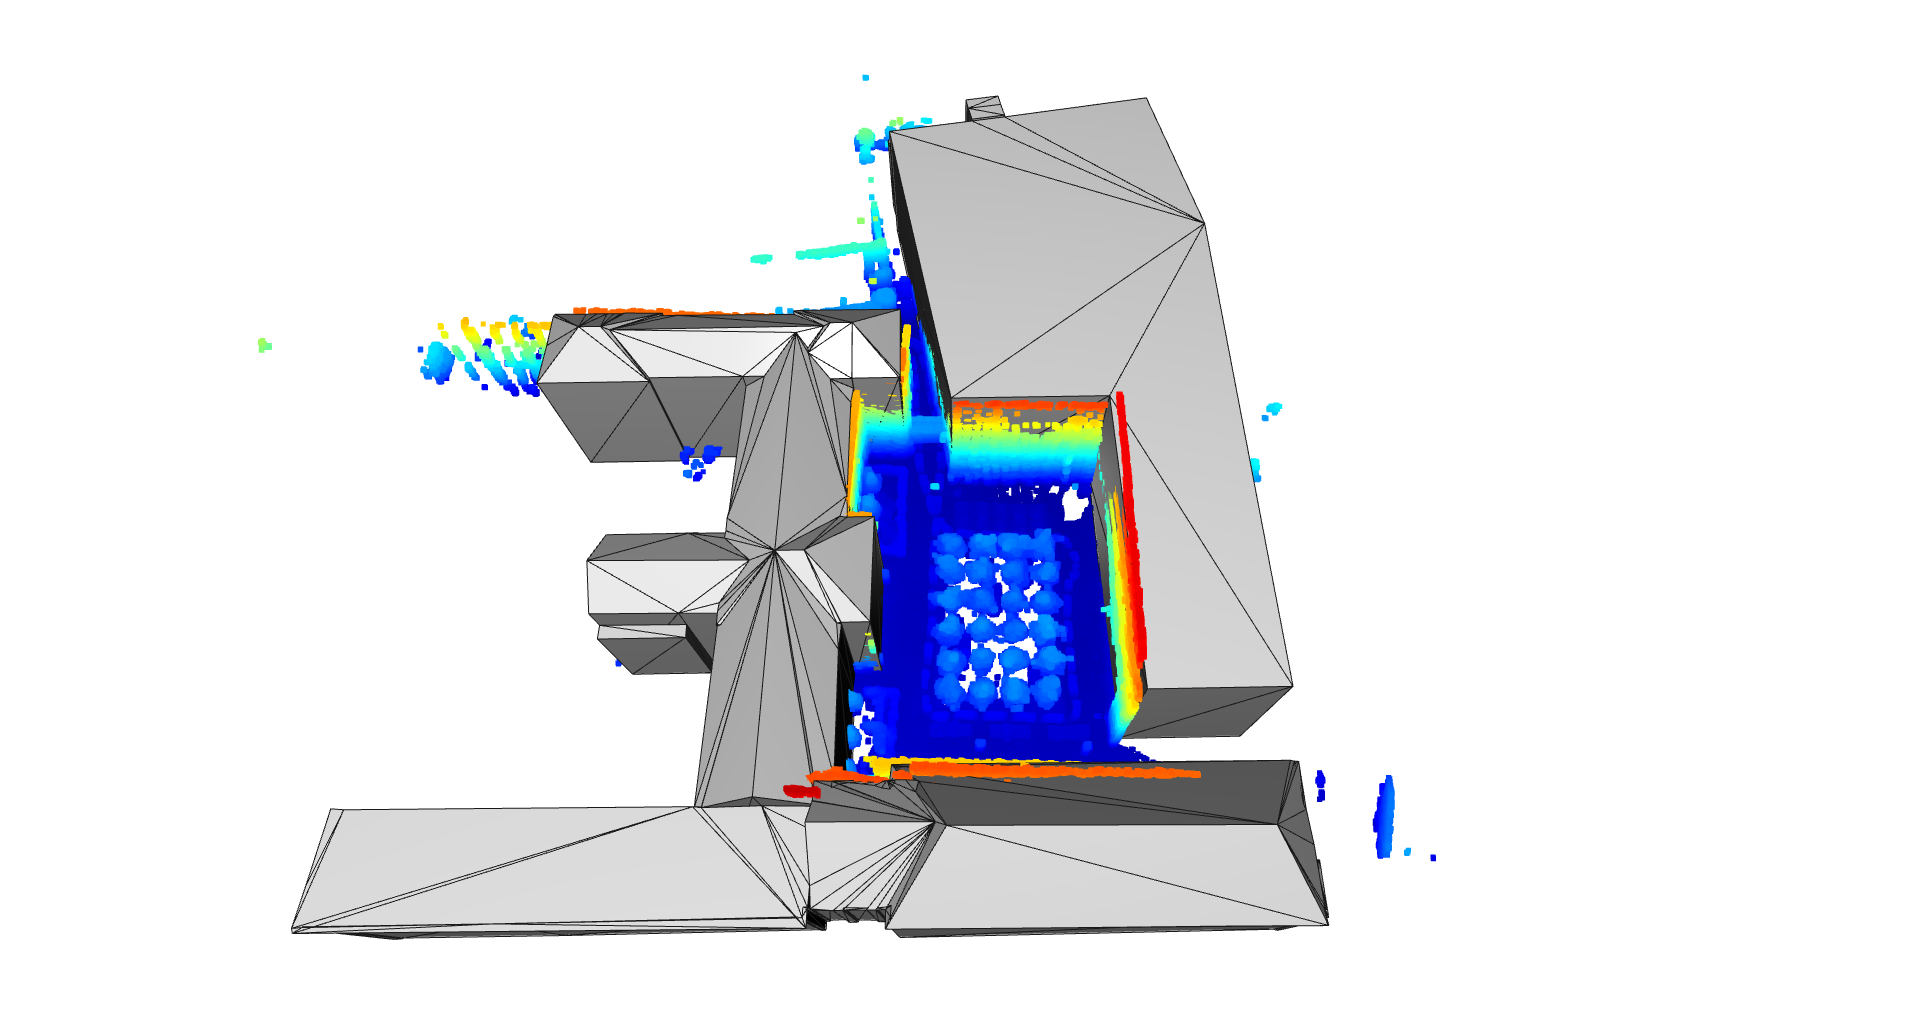
\includegraphics[scale=0.15]{images/solution_images/final_ply_b.png}
                \caption{Second view.}
                \label{fig:final_ply_b}
            \end{subfigure}
            \caption{PLY model and its corresponding point cloud after registration.}
            \label{fig:final_ply}
        \end{figure}

%-------------------------------------------------------------------------------
%	Discussion
%-------------------------------------------------------------------------------
    \section{Discussion}
        The results presented in the two past sections highly depend on the step described in 
        \autoref{sub:Detection of line intersections and their angles}, i.e., on detecting lines and their intersections.
        If the number of intersections detected is poor, then the registration results could be wrong.
        Furthermore, the accuracy of the registration result depends on the accuracy with which the position of the intersections is detected.
        Therefore, if no lines and no intersections are detected, then no registration is possible.

        The different running times presented in \autoref{table:running_time} could be due to the size of the point clouds. 
        The point cloud corresponding to the CityGML model contains 1178841 points before being downsampled and 1159064 points after being downsampled.
        In contrast, the point cloud corresponding to the PLY model contains 3724578 points before being downsampled and 2805065 points after being downsampled.

        Furthermore, the number of intersections detected in the projections onto the xy-plane, both of the models and the point clouds, differs too.
        The number of intersections detected in the projection of the CityGML model and its corresponding point cloud is 3 and 39, respectively. 
        In comparison, the number of intersections detected in the projection of the PLY model and its corresponding point cloud is 10 and 43, respectively.
        Therefore, the Mixed Integer Linear Program takes longer for the PLY model.
        
        

% % % % % % % % CityGML
% % % % % % % % PointCloud with 1178841 points.
% % % % % % % % Downsampling
% % % % % % % % PointCloud with 1159064 points.
% Point cloud: Number of corners: 3
% Model: Number of corners: 39

% % % % % % % % PLY
% % % % % % % % PointCloud with 3724578 points.
% % % % % % % % Downsampling
% % % % % % % % PointCloud with 2805065 points.

% Point cloud: Number of corners: 10
% Model: Number of corners: 43

        

    
\end{document}
